% Reviewer 1
\reviewer

% ---- Comment 1.1 ----
\begin{revcomment}
	The data-collection model is overly simplified. Although each GN has a certain data volume, successful collection is determined only by the path-loss threshold and the prescribed duration $\tau_i$, without explicitly modeling achievable rate, bandwidth, SINR, or data size.
\end{revcomment}

\begin{revresponse}[]
	Thank you for this valuable comment. We agree that the previous formulation left the relationship between the prescribed collection duration $\tau_i$ and the underlying data-collection process implicit. We have revised the system model to explicitly incorporate the achievable rate, the bandwidth, the SINR, and the data volume, and to tie the successful-collection condition to these quantities.

	\textbf{(1) Nominal SINR and achievable rate.} In the revised Section~3.1, we characterize each $GN_i$ by a nominal SINR $\Gamma_i$, a per-node parameter analogous to the path-loss threshold $PL_i^{max}$; the achievable rate is evaluated at this nominal SINR through the Shannon capacity, $\bar{R}_i=B\log_2(1+\Gamma_i)$, where $B$ is the channel bandwidth.

	\textbf{(2) Constant-rate characterization.} Since $\Gamma_i$ is fixed, the achievable rate $\bar{R}_i$ is constant throughout the collection phase, so the collection duration $\tau_i=D_i/\bar{R}_i$ remains a fixed per-node quantity; this constant-rate characterization keeps the problem tractable and preserves the fixed-$\tau_i$ structure that enables the stage-wise dynamic-programming optimality analysis.

	\textbf{(3) Successful-collection condition.} Given the data volume $D_i$ of $GN_i$, the required collection duration is now explicitly $\tau_i=D_i/\bar{R}_i$, and the collection of $GN_i$ is defined to be successful if and only if the UAV stays within its communication region for a total duration of at least $\tau_i$. This connects the path-loss threshold (which defines the coverage region) to the data volume, bandwidth, and SINR through the achievable rate, while preserving the fixed-$\tau_i$ structure of the problem.

	The simulation setup is updated accordingly: $B=1$ MHz, $\Gamma_i$ sampled per GN from $[12,18]$ (default $15$), and $D_i$ averaged $88$ Mbit with range $[72,100]$ Mbit, so that $\tau_i=D_i/\bar{R}_i\approx22$ s on average (matching the original configuration).

	The revised text in the manuscript is as follows.
	\begin{changes}
		\textbf{Section~3.1 (added).} To model the data upload, we characterize each $GN_i$ by a nominal SINR $\Gamma_i$, a per-node parameter analogous to the path-loss threshold $PL_i^{max}$. Letting $B$ denote the channel bandwidth, the achievable rate of the link is evaluated at this nominal SINR through the Shannon capacity:
		\begin{equation*}
			\bar{R}_i = B\log_2(1+\Gamma_i).
		\end{equation*}
		Each $GN_i$ therefore uploads data at the constant rate $\bar{R}_i$ throughout the collection phase, which yields the deterministic collection duration $\tau_i = D_i/\bar{R}_i$.

		\textbf{Section~3.3 (revised Definition).} Given ordered ground nodes $GN_1,\ldots,GN_N$, their communication regions, and the data volume $D_i$ of each $GN_i$, the \textit{JHVSO} problem seeks a trajectory $q(t)=(d(t),h(t))$ and collection intervals that minimize the total flight energy. Under the constant achievable rate $\bar{R}_i$, collecting the data volume $D_i$ requires a duration $\tau_i=D_i/\bar{R}_i$; the collection of $GN_i$ is successful if and only if the UAV stays within its communication region for a total duration of at least $\tau_i$.

		\textbf{Table~1 (revised).} The row ``Average $\tau$ (s) 22 [18 25]'' is replaced by ``Average $D_i$ (Mbit) 88 [72 100]'', and a new row ``Nominal SINR $\Gamma_i$ 15 [12 18]'' is added.

		\textbf{Section~6 (added).} The data upload adopts a channel bandwidth of $B=1$ MHz and a per-GN nominal SINR $\Gamma_i$ sampled from $[12,18]$ (default $15$), which yields a constant achievable rate $\bar{R}_i=B\log_2(1+\Gamma_i)$, about $4$ Mbps at the default; the required collection duration is then $\tau_i=D_i/\bar{R}_i$, approximately $22$ s on average under the default data volume $D_i=88$ Mbit.

		\textbf{Figure~2 (revised caption).} The UAV must remain within the region of $GN_i$ for the required data collection duration $\tau_i=D_i/\bar{R}_i$, where $D_i$ is the data volume of $GN_i$ and $\bar{R}_i=B\log_2(1+\Gamma_i)$ is the constant achievable rate.
	\end{changes}
\end{revresponse}

% ---- Comment 1.2 ----
\begin{revcomment}
	The claimed coupling between horizontal and vertical propulsion is not sufficiently reflected in the model as shown in Eq. (3). The total power is formulated as the additive form. The authors should clarify what physical coupling is actually captured.
\end{revcomment}

\begin{revresponse}[]
	Thank you for this comment. We agree that the horizontal and vertical power models are additive and therefore do not exhibit a coupling between the two power components; the earlier phrase ``continuous coupling between horizontal and vertical propulsion power'' was an imprecise wording, which we have now corrected throughout the manuscript.

	To state the relationship between the two velocity components precisely, we have revised the total power model in Eq.~(4) to express it directly in terms of the total flight speed $V_{total}$ and the flight pitch angle $\gamma$:
	\[
		P_{total}(V_{total}) = P_{mh} + \Delta P_{\parallel}(V_{total}\cos\gamma) + \Delta P_{\perp}(V_{total}\sin\gamma),
	\]
	where the horizontal and vertical velocity components appear explicitly as $V_{total}\cos\gamma$ and $V_{total}\sin\gamma$. This makes clear how the two components combine into the total speed and, through the additive power model, into the total power. Accordingly, the wording ``coupling between horizontal and vertical propulsion power'' has been replaced by ``joint horizontal--vertical speed optimization''.

	The revised text is as follows.
	\begin{changes}
		\textbf{Abstract (revised).} To capture realistic three-dimensional motion, we adopt a practical 3D flight energy consumption model and jointly optimize the horizontal and vertical speeds.

		\textbf{Introduction (revised).} Instead of optimizing horizontal speed and height separately, we focus on joint horizontal-vertical speed optimization.

		\textbf{Related work (revised).} However, existing 3D extensions typically schedule the two dimensions independently (e.g., as discrete altitude transitions). In contrast, our formulation retains the additive instantaneous-power form of [11,12] but jointly optimizes the two speed components through the flight pitch angle, as detailed in Section 3.2.

		\textbf{Section~3.2 (revised Eq.~(4)).} Let $V_{total}$ denote the total (resultant) flight speed and $\gamma$ the flight pitch angle, defined as the angle between the velocity vector and the horizontal plane. The total power is then expressed directly in terms of these two quantities:
		\[
			P_{total}(V_{total}) = P_{mh} + \Delta P_{\parallel}(V_{total}\cos\gamma) + \Delta P_{\perp}(V_{total}\sin\gamma).
		\]
	\end{changes}
\end{revresponse}

% ---- Comment 1.3 ----
\begin{revcomment}
	Regarding the Theorem in Section 3.2, the resulting trajectory may not be dynamically feasible for a physical UAV. Consecutive flight segments can have different velocities at their shared boundary, effectively requiring instantaneous velocity changes. The authors should discuss whether such piecewise constant-speed trajectories can be practically tracked and consider incorporating acceleration constraints or transition dynamics into the model.
\end{revcomment}

\begin{revresponse}[]
	Thank you for this comment. The optimal trajectory is indeed piecewise constant-speed, so consecutive segments may differ in velocity at their shared boundary. We have clarified this point in the revised manuscript as follows.

	The constant segment speeds should be interpreted as target cruise speeds, which a physical UAV tracks with short acceleration/deceleration ramps. The time and energy consumed during these transition phases account for only a small fraction of the total mission time and energy~\cite{msmo}, so they do not materially affect the planned schedule or the energy-optimal speed selection. We have added a remark in Section~4.1 stating this explicitly; incorporating full acceleration dynamics into the optimality analysis is left as future work, consistent with the existing limitation in the conclusion.

	The revised text is as follows.
	\begin{changes}
		\textbf{Section~4.1 (added Remark).} The resulting trajectory is piecewise constant-speed, with task segments flown per Remark 1 and gap segments per Theorem 2, so consecutive segments may change velocity at their shared boundary. In practice, this change is realized by a brief acceleration/deceleration phase whose time and energy are only a small fraction of the total mission~\cite{msmo}; the constant speeds are therefore target cruise speeds tracked with short transition ramps, and full acceleration dynamics are left as future work. 
    \end{changes}
\end{revresponse}

% ---- Comment 1.4 ----
\begin{revcomment}
	Wind and other environmental disturbances are ignored. Since propulsion power depends on airspeed while trajectory progression depends on ground speed, wind may significantly affect both the energy consumption and the optimal speed schedule.
\end{revcomment}

\begin{revresponse}[]
	Thank you for this insightful comment. We agree that wind changes the airspeed relative to the ground speed, and thus affects both the propulsion power and the energy-optimal speed schedule. The present work is scoped to nominal, wind-free conditions, under which the ground speed equals the airspeed, so the propulsion power and the energy-optimal speed schedule remain as modeled. Explicitly incorporating wind and stochastic channel conditions is a valuable direction for future work; to keep the manuscript focused and within the page limit, we address this limitation in this reply rather than adding a dedicated passage to the paper. But we regard it as an important future direction.

\end{revresponse}

% ---- Comment 1.5 ----
\begin{revcomment}
	The claimed global optimality is only guaranteed over the discretized state space. The manuscript should provide a sensitivity study on the discretization resolution, energy convergence, and computational cost. But we regard it as an important future direction.
\end{revcomment}

\begin{revresponse}[]
	Thank you for this important comment. We have addressed it in two respects: we have qualified the global-optimality claim throughout the manuscript, and we have added a dedicated sensitivity study.

	\textbf{(1) Qualifying the optimality claim.} All optimality statements are now explicitly scoped to the discretized state space. In particular, the abstract and Theorem~4 state that the ORE algorithm guarantees global optimality \emph{over the discretized state space}, and the conclusion no longer claims optimality over the continuous trajectory design.

	\textbf{(2) Sensitivity study.} We have added a new Section~6.3, \emph{Discretization Sensitivity and Computational Cost}, which varies the state sampling cap $M\in\{250,500,1000,2000,4000\}$ and reports the total energy of each experiment under each cap in a new table, together with the running time and the relative optimality gap (new Fig.~9).

	\textbf{(3) Findings.} The optimal energy decreases monotonically and converges as $M$ grows: refining $M$ from $1000$ to $4000$ reduces the energy by only $0.14\%$, and the improvement roughly halves whenever the resolution doubles, indicating first-order convergence. At the operating resolution $M=2000$, the optimal energy is within $0.07\%$ of that at $M=4000$, at an average running time of $4.86$ s. Hence a sampling cap in the range $M\in[1000,2000]$ provides a good balance between optimality and computational cost, confirming that the discretized optimum has essentially converged to the continuous optimum.

	The added text in the revised manuscript is as follows.
	\begin{changes}
		\textbf{Section~6.3 (added).} The global optimality guarantee of the proposed ORE algorithm holds over the discretized state space, i.e., over the finite set of candidate states sampled within the communication region of each GN. Concretely, the continuous communication region of each GN is first rasterized onto a fine grid in the $(d,h)$ plane with a resolution of $1$ m, which yields the full set of candidate state points located inside the coverage region. When a GN contains more candidate points than a prescribed cap $M$, the points are uniformly subsampled in raster order---keeping every $s$-th point with $s=\lfloor N_c/M\rfloor$, where $N_c$ is the number of candidate points of that GN---so that approximately $M$ states remain; GNs whose coverage contains no more than $M$ candidate points keep all of them. As a result, the actual number of sampled states of each GN fluctuates around $M$ depending on its coverage area (on average approximately $2357$ and $5791$ states for $M=2000$ and $M=4000$, respectively). To assess the impact of this sampling resolution, we evaluate the algorithm under different caps $M\in\{250,500,1000,2000,4000\}$. The total energy (J) and the relative improvement (\%) of each experiment under each cap are reported in a new table (Table~2 in the manuscript), shown here in its two parts:

\textbf{Total energy (J):}
\begin{center}
\small
\begin{tabular}{lccccc}
\toprule
 & $M=250$ & $M=500$ & $M=1000$ & $M=2000$ & $M=4000$ \\
\midrule
 Exp.\ 1 & 153946 & 153558 & 153370 & 153315 & 153178 \\
 Exp.\ 2 & 162798 & 162207 & 162005 & 161858 & 161742 \\
 Exp.\ 3 & 151038 & 150486 & 150338 & 150171 & 150078 \\
 Exp.\ 4 & 153148 & 152940 & 152693 & 152600 & 152535 \\
 Exp.\ 5 & 155466 & 155100 & 155092 & 155001 & 154873 \\
\midrule
 Mean & 155279 & 154858 & 154700 & 154589 & 154481 \\
\bottomrule
\end{tabular}
\end{center}

\textbf{Relative improvement (\%):}
\begin{center}
\small
\begin{tabular}{lcccc}
\toprule
 & $250\!\to\!500$ & $500\!\to\!1000$ & $1000\!\to\!2000$ & $2000\!\to\!4000$ \\
\midrule
 Exp.\ 1 & 0.2520 & 0.1224 & 0.0361 & 0.0895 \\
 Exp.\ 2 & 0.3630 & 0.1243 & 0.0907 & 0.0717 \\
 Exp.\ 3 & 0.3657 & 0.0982 & 0.1107 & 0.0625 \\
 Exp.\ 4 & 0.1363 & 0.1612 & 0.0609 & 0.0428 \\
 Exp.\ 5 & 0.2359 & 0.0052 & 0.0584 & 0.0824 \\
\midrule
 Mean & 0.2706 & 0.1023 & 0.0714 & 0.0698 \\
\bottomrule
\end{tabular}
\end{center}

		As shown in the new table, the total energy of every experiment decreases monotonically and converges as $M$ increases: on average, refining $M$ from $1000$ to $4000$ reduces the total energy by only $0.14\%$, and the improvement shrinks as the resolution doubles, indicating approximately first-order convergence (Fig.~9(b)). At the operating resolution $M=2000$, the optimal energy is within $0.07\%$ of that obtained at $M=4000$; this residual gap reflects the discretization error of the state space and is negligible in practice, confirming that the discretized optimum has essentially converged to the continuous optimum. Meanwhile, as shown in Fig.~9(a), the running time grows with $M$, averaging $4.86$ s at the operating resolution $M=2000$. Overall, a sampling cap in the range $M\in[1000,2000]$ strikes a good balance between energy optimality and computational cost. This confirms that the global-optimality guarantee over the discretized state space carries over to the continuous problem with negligible loss.

		\begin{center}
			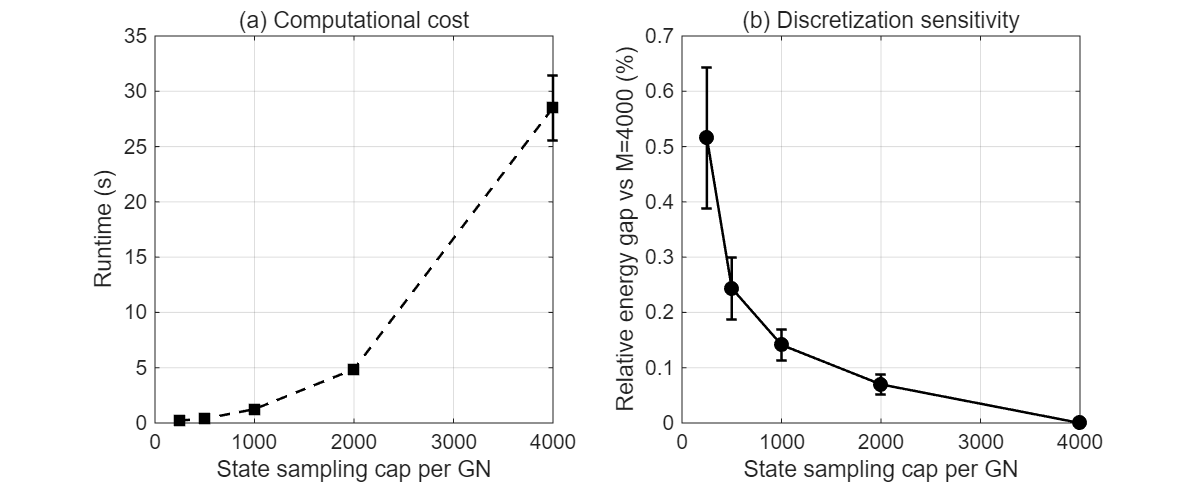
\includegraphics[width=1\linewidth]{figures/discretization-sensitivity.png}
		\end{center}

		\textbf{Figure 9 (added).} Discretization sensitivity and computational cost: (a) running time and (b) the relative optimality gap versus the state sampling cap $M$.

		\textbf{Section~7 (added sentence).} A sensitivity study further confirms that the discretized optimum converges to the continuous optimum with negligible loss (within $0.07\%$ at the operating resolution).
	\end{changes}
\end{revresponse}

\printpartbibliography{msmo}
